\documentclass[tikz,border=6pt]{standalone}
\usetikzlibrary{arrows.meta}

\begin{document}
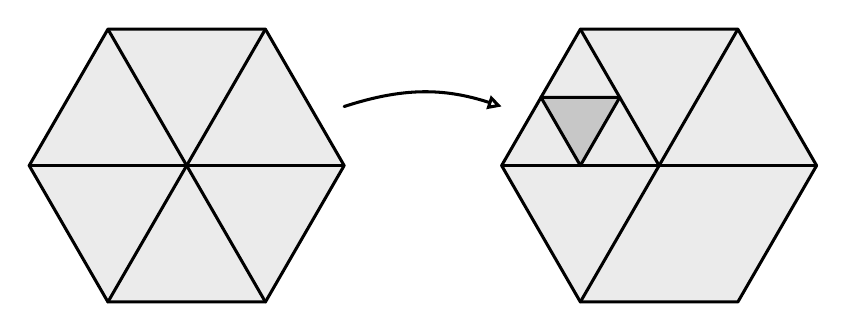
\begin{tikzpicture}[
    line width=1.1pt,
    line join=round,
    line cap=round,
    cell/.style={fill=black!8},
    marked/.style={fill=black!22},
  ]

  %% ------------------------------------------------------------------
  %% left hexagon: uniform macro-triangulation
  %% ------------------------------------------------------------------
  \begin{scope}[shift={(0,0)}]
    \coordinate (aC)  at ( 0      , 0       );
    \coordinate (aL)  at (-2      , 0       );
    \coordinate (aTL) at (-1      , 1.73205 );
    \coordinate (aTR) at ( 1      , 1.73205 );
    \coordinate (aR)  at ( 2      , 0       );
    \coordinate (aBR) at ( 1      ,-1.73205 );
    \coordinate (aBL) at (-1      ,-1.73205 );

    % shading (all six triangles)
    \path[cell] (aL) -- (aTL) -- (aTR) -- (aR) -- (aBR) -- (aBL) -- cycle;

    % edges (each drawn exactly once)
    \draw (aL) -- (aTL) -- (aTR) -- (aR) -- (aBR) -- (aBL) -- cycle;
    \draw (aL)  -- (aR);
    \draw (aTL) -- (aBR);
    \draw (aTR) -- (aBL);
  \end{scope}

  %% ------------------------------------------------------------------
  %% arrow
  %% ------------------------------------------------------------------
  \draw[-{Triangle[open,length=5pt,width=5pt]}]
        (2,0.75) to[bend left=18] (4,0.75);

  %% ------------------------------------------------------------------
  %% right hexagon: locally refined / partially deactivated
  %% ------------------------------------------------------------------
  \begin{scope}[shift={(6,0)}]
    \coordinate (bC)  at ( 0      , 0       );
    \coordinate (bL)  at (-2      , 0       );
    \coordinate (bTL) at (-1      , 1.73205 );
    \coordinate (bTR) at ( 1      , 1.73205 );
    \coordinate (bR)  at ( 2      , 0       );
    \coordinate (bBR) at ( 1      ,-1.73205 );
    \coordinate (bBL) at (-1      ,-1.73205 );

    % edge midpoints of the refined upper-left triangle
    \coordinate (bM1) at (-1.5    , 0.866025);
    \coordinate (bM2) at (-0.5    , 0.866025);
    \coordinate (bM3) at (-1      , 0       );

    % shading: upper half + lower-left triangle
    \path[cell] (bL) -- (bTL) -- (bTR) -- (bR) -- (bC) -- cycle;
    \path[cell] (bL) -- (bC)  -- (bBL) -- cycle;
    \path[cell] (bL) -- (bTL) -- (bTR) -- (bR) -- (bBR) -- (bBL) -- cycle;
    \path[marked] (bM1) -- (bM2) -- (bM3) -- cycle;

    % edges (each drawn exactly once)
    \draw (bL) -- (bTL) -- (bTR) -- (bR) -- (bBR) -- (bBL) -- cycle;
    \draw (bL)  -- (bR);
    \draw (bTL) -- (bC);
    \draw (bTR) -- (bC);
    \draw (bBL) -- (bC);

    % local refinement of the upper-left triangle
    \draw (bM1) -- (bM2) -- (bM3) -- cycle;
  \end{scope}

\end{tikzpicture}
\end{document}
